\documentclass[10pt,compress]{beamer}
    \useoutertheme{miniframes}
    \usepackage[english]{babel}
    %\usepackage[margin=1in]{geometry}

    \usepackage{amsmath}
    \usepackage{amsfonts} 
    \usepackage{amssymb}
    \usepackage{amsthm}
    \usepackage{mathtools}

    \usepackage[utf8]{inputenc}
    %\usepackage[exscale, amsfonts, amssymb]{concmath}
    %\renewcommand*{\bfseries}{\mdseries}

    \usepackage{float}
    \usepackage{graphicx}
    \usepackage{caption}
    \usepackage{subcaption}

    \graphicspath{{./src/figures/}}

    %\usepackage{fancyhdr} %custom headers and footers layout
    \usepackage{lastpage} %package to print the last page
    %\pagestyle{fancy} %fancy page style

    \usepackage{textcomp} 
    \usepackage{multicol} 
    \usepackage{multirow}

    \usepackage[table]{xcolor}
    \usepackage{booktabs}

    \usepackage[backend=biber,
    bibstyle=ieee, 
    citestyle=numeric-comp,
    natbib=true,
    doi=false, 
    url=false,
    isbn=false,
    mincitenames=1,
    maxcitenames=1,
    minbibnames=1,
    maxbibnames=99,
    backref=false,]
    {biblatex}
    \addbibresource[label=main]{./src/references.bib}

    \usepackage{url}
    \usepackage{hyperref}

    %edit the properties of your PDF documents which will be displayed
    \hypersetup{
        bookmarks=true, 		% show bookmarks bar?
        unicode=true,  		% non-Latin characters in Acrobat’s bookmarks
        pdftoolbar=true,        % show Acrobat’s toolbar?
        pdfmenubar=true,        % show Acrobat’s menu?
        pdffitwindow=true,      % page fit to window when opened
        pdftitle={PhotoElectrochemistry --- Theoretical Background},    % title
        pdfauthor={M. Skocic},     % author
        pdfsubject={},   % subject of the document
        pdfnewwindow=true,      % links in new window
        pdfkeywords={}, % list of keywords
        colorlinks=false,       % false: boxed links; true: colored links
        linkcolor=red,          % color of internal links
        citecolor=green,        % color of links to bibliography
        filecolor=magenta,      % color of file links
        urlcolor=cyan           % color of external links
    }

    \usepackage{tikz}
    \usepackage{circuitikz}
    \usetikzlibrary{decorations.pathmorphing,arrows,calc}

    \title{PhotoElectroChemistry for Corrosion}
    \author{M. Skocic, PhD Electrochemistry and Materials}
    \date{\vfill 
\includegraphics[width=0.70\textwidth]{full_bw.png}}

    \newcommand{\coef}{1}

\begin{document}
    \begin{frame}
        \titlepage
    \end{frame}

    \begin{frame}
        \frametitle{Contents}
        \tableofcontents
    \end{frame}


% INTRODUCTION
\section{Introduction}
    \begin{frame}{Introduction}
        \begin{itemize}
            \item Photoelectrochemical techniques have been shown to be useful tools for characterizing oxidation layers. 
            \item Interdisciplinary theoretical underpinnings were built \citep{morrison1980, vijh1969, stimming1986, diquarto1997, wouters2007} 
                  such as the Gärtner-Butler model \citep{gartner1959,butler1977}
                  which has been proven to be a simple and robust model for the photocurrent generation. 
            \item Technical progresses were achieved, allowing to study oxide layers at 
                  macroscopic, mesoscopic, and microscopic scales 
                  \citep{benaboud2007, srisrual2011}, or in-situ in high temperature corrosion 
                  conditions \citep{bojinov2002,skocic2016}.
        \end{itemize}
    \end{frame}

    \begin{frame}{Hypotheses}
        Several hypotheses are needed in order to apply the theoretical concepts:  
        \begin{itemize}
            \item semiconductors are considered to be ideal i.e. crystallized and homogeneous  
            \item the dielectric constant of the semiconductor is independent of the light wavelength  
            \item the capacity of the Helmholtz layer is greater than the capacitance of the space charge capacitance  
            \item the potential drop in the Helmholtz layer is independent of the applied potential and is negligible
        \end{itemize}

        \footnotesize
        \begin{alertblock}{Warning}
            The hypotheses are rarely fully respected in the case of oxides or passive 
            films formed on industrial alloys. Nonetheless, the literature shows that the 
            developed models can be applied to non-ideal systems such as oxides 
            and passive films.
        \end{alertblock}
    \end{frame}



% BASICS
\section{basics}
\subsection{Electronic Band Structure}
    \begin{frame}[allowframebreaks=1.0]{Band Model}
        \begin{itemize}
            \item Solids: conductors, semiconductors and insulators. 
            \item Valence and conduction bands correspond to allowed energy states for the electrons. 
            \item $E_c$ is the lowest energy level of the conduction band.
            \item $E_v$ is the highest energy level of the valence band.
            \item $E_g$ is the band gap with no allowed energy states. 
            \item $E_F$ is the Fermi Level which describes the distribution of the electrons among both bands.
        \end{itemize}
        
        \begin{alertblock}{Fermi Level}
            \footnotesize
            The Fermi Level represents the highest energy state that can be occupied level at 0K. 
            It is equivalent to the electrochemical potential in solid phases.
        \end{alertblock}
        
        \framebreak
        \begin{itemize}
            \item The electronic conduction = movement of electrons and/or holes in conduction/valence band.
            \item The conduction depends on the number of available charge carriers
            in the conduction band and in the valence band. 
            \item In conductors: overlap of the conduction and the valence bands occurs. 
            \item In semiconductor and insulator: the conduction depends on the band gap and the energy provided by 
            the environment to the electrons from the valence band in order to jump 
            into the conduction band.
        \end{itemize}

        \begin{figure}[h]
            \centering
                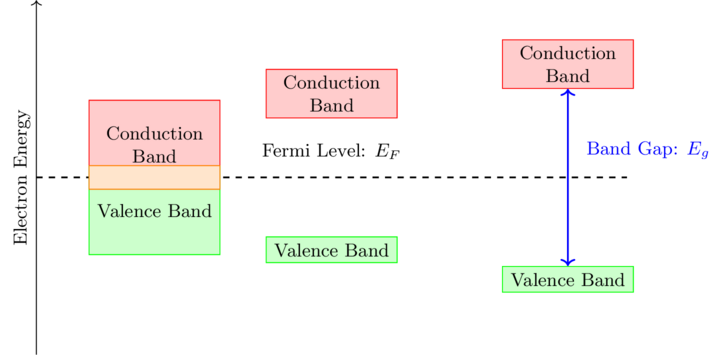
\includegraphics[width=0.65\textwidth]{tikz_band_model.png}
            %\caption{Schematic representation of the electronic band structure \citep{marucco2006}: 
            %a) conductor, b) semiconductor, c) insulator}
            \label{fig_band_model}
        \end{figure}
    \end{frame}

    \begin{frame}[allowframebreaks=1.0]{Excitation carrier}
        In semiconductors, charge carriers can be generated by three mechanisms: 
        \begin{itemize}
            \item thermal excitation: in the case of very low band gaps, it can be enough in order 
            to eject an electron from $E_v$ to $E_c$.
            \item photoexcitation: ejects electrons from $E_v$ to $E_c$
            band when an incident photon ($h\nu > 5eV$) is absorbed.
            \item doping: introduces additional energy level located in between $E_v$ to $E_c$.
        \end{itemize}
        
        \begin{figure}[h]
            \centering
            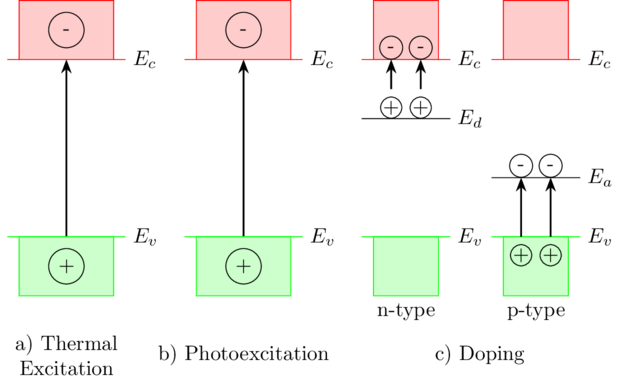
\includegraphics[width=0.6\textwidth]{tikz_excitation_carrier.png}
            %\caption{Schematic representation of the mechanisms generating charge carriers in semiconductors \citep{finklea1983}: 
            %a) thermal excitation, b) photoexcitation, c) doping}
            \label{fig_excitation_carrier}
        \end{figure}
    \end{frame}

    \begin{frame}{Fermi Position}
        The Fermi level $E_F$ in intrinsic semiconductors is located at the mid-gap. 
        The n-type and p-type doping shift the Fermi level towards band edges 
        $E_c$ and $E_v$.
        \begin{figure}[H]
            \centering
            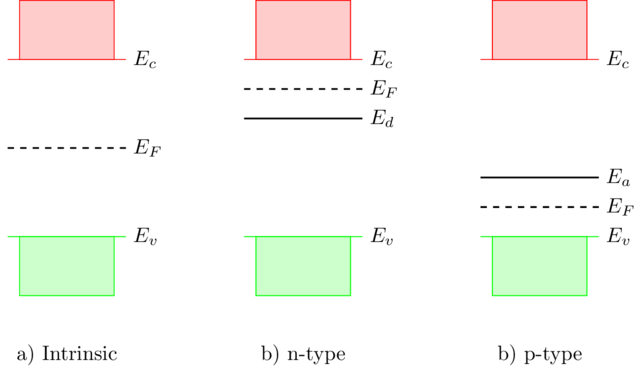
\includegraphics[width=0.65\textwidth]{tikz_fermi_position.png}
            %\caption{Schematic representation of the Fermi level with respect to the 
            %semiconduction type \citep{finklea1983}: a) intrinsic, b) n-type, c) p-type.}
            \label{fig_fermi_position}
        \end{figure}
    \end{frame}

\subsection{Semiconductor/electrolyte interface in dark condition}

\subsection{Semiconductor/electrolyte interface under illumination}
    \begin{frame}[allowframebreaks=1.0]{Electron/hole pairs}
    \begin{itemize} 
        \item The illumination of the semiconductor/electrolyte interface, 
        with photons having an energy greater than the band gap, $E_g$, creates 
        electron/hole pairs in the semiconductor. 
        \item By applying the adequate potential the pairs can be separated. 
        \item As a consequence, the majority charge carriers are attracted to the 
        semiconductor bulk whereas the minority charge carriers are drawn to the 
        semiconductor/electrolyte interface where they can be transferred to a RedOx 
        species creating an additional current called photocurrent. 
    \end{itemize}
    
    \begin{figure}[h]
        \centering
        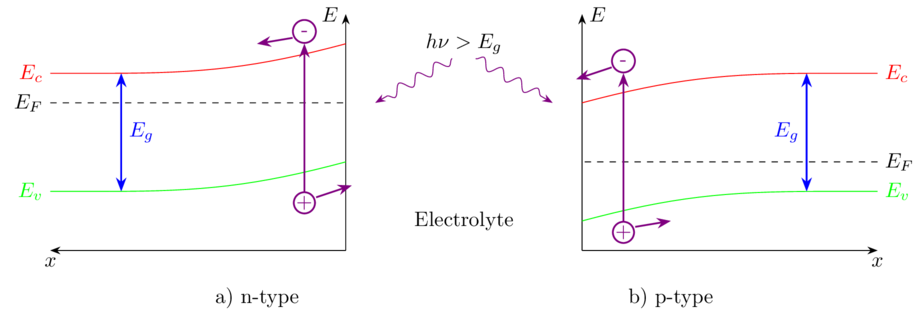
\includegraphics[width=0.65\textwidth]{tikz_photocurrent_generation.png}
        %\caption{Schematic representation of the mechanism generating 
        %a photocurrent \citep{memming2008,bard2002}.}
        \label{fig_photocurrent_generation}
    \end{figure}
    
    \begin{itemize}
        \item The photocurrent is significant when the semiconductor/electrolyte junction 
        is in depletion. 
        \item n-type (p-type) 
        semiconductors generate anodic (cathodic) photocurrents where the 
        electrons (holes) move towards the external circuit whereas the holes (electrons) 
        move towards the interface. 
        \item The applied potential on n-type (p-type) semiconductors is 
        greater (lower) than the flat band potential. \index{potential!flat band}
    \end{itemize}

    \begin{figure}[h]
        \centering
        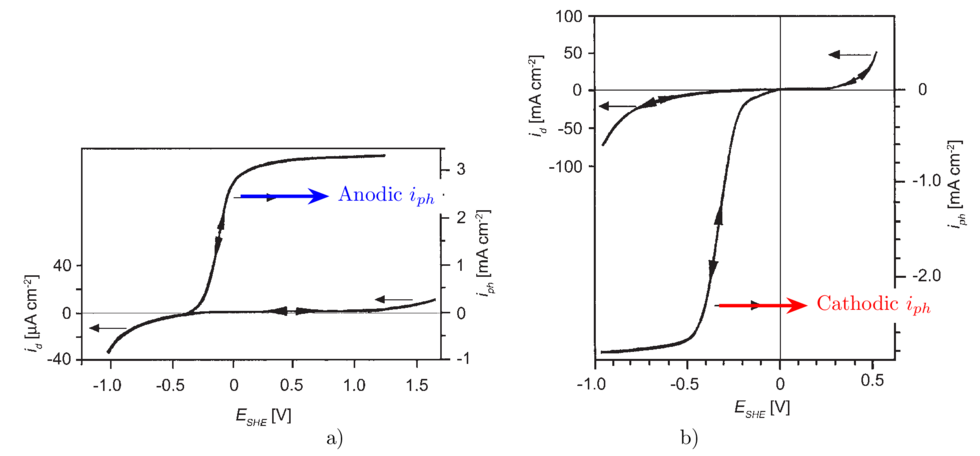
\includegraphics[width=0.65\textwidth]{tikz_photocurrent_plieth.png}
        %\caption{Photocurrent density $i_{ph}$ and dark current density 
        %$i_d$ with respect to the potential in a case of GaAs semiconductor 
        %\citep{plieth2008}: a) n-type, b) p-type.}
        \label{fig_photocurrent_plieth}
    \end{figure}

    \end{frame}


    \begin{frame}[allowframebreaks=1.0]{Linear transform}
        \begin{itemize}
            \item The linear transform with respect to the energy is used for determining the band gaps. 
            \item The linear transform with respect to the potential  is used for determining 
                  the semiconducting type, the flat band potential, 
                  and the number of majority charge carrier.
        \end{itemize}
    \end{frame}



% APPLICATIONS 
\section{Applications}
\subsection{Minor oxides}
    \begin{frame}[allowframebreaks=1.0]{Identification of minor oxides}
        \begin{itemize}
            \item \citet{benaboud2007} showed that the photoelectrochemical characterization 
                  is robust for detecting the presence of minor oxides. 
            \item The strong photocurrent observed at around 5~eV 
                  reveals the major oxide i.e. monoclinic zirconia. 
            \item The photocurrent $h\nu < 5 eV$ reveals the presence of minor 
                  oxides even in “pure” zirconium. 
            \item The slope changes provided an estimation of the band gaps: 
                  hematite, chromia and a solid solution of $(Fe_xCr_{1-x})O_3$. 
        \end{itemize}

        \renewcommand{\coef}{0.45}
        \begin{figure}[h]
            \centering
            \begin{subfigure}{\coef\textwidth}
                \centering
                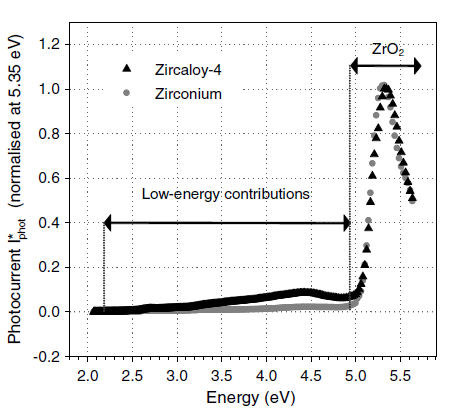
\includegraphics[width=0.65\textwidth]{./src/figures/Benaboud2007-Fig4.png}
                \caption{}
                \label{fig_benaboud_minor_oxides_a}
            \end{subfigure}
            \begin{subfigure}{\coef\textwidth}
                \centering
                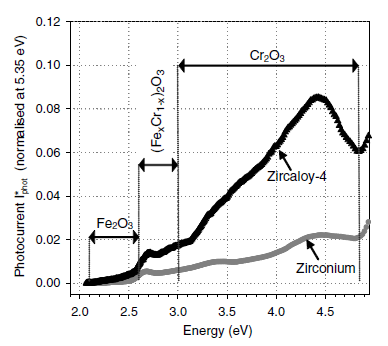
\includegraphics[width=0.65\textwidth]{./src/figures/Benaboud2007-Fig5.png}
                \caption{}
                \label{fig_benaboud_minor_oxides_b}
            \end{subfigure}
            
            %\caption{Photocurrent spectra measured on zirconia oxide layer formed on 
            %Zircaloy4 and “pure” zirconium oxidized for 1h at 470°C in oxygenated 
            %atmosphere\citep{benaboud2007}: a) complete spectrum b) close-up view on the minor contributions.}
            \label{fig_benaboud_minor_oxides}
        \end{figure}
    \end{frame}

\subsection{Semiconducting type}
    \begin{frame}[allowframebreaks=1.0]{Semiconduction type}
        \begin{itemize}
            \item \citet{loucif2013} showed the effect of hydrogen pressure on 
                  the semiconduction type on Ni-based alloy 600 oxidized in simulated PWR. 
            \item The “V-shape” of the normalized photocurrent 
                  reveals an isolating behavior of the oxide layer at high hydrogen pressure. 
            \item The monotonous increase of the 
                  normalized photocurrent towards more anodic potentials reveals 
                  n-type semiconduction.
        \end{itemize}

        \renewcommand{\coef}{0.45}
        \begin{figure}[h]
            \centering
            \begin{subfigure}{\coef\textwidth}
                \centering
                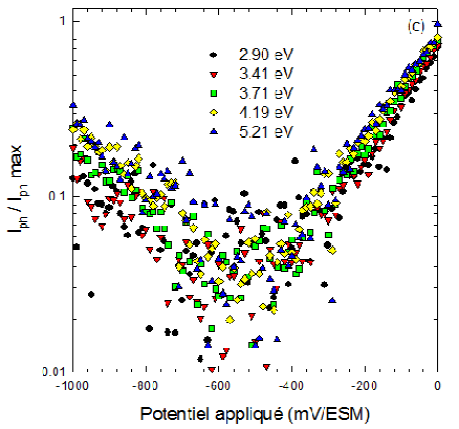
\includegraphics[width=0.65\textwidth]{./src/figures/Loucif2012-Fig3-18.png}
                \caption{}
                \label{fig_loucif_sctype_a}
            \end{subfigure}
            \begin{subfigure}{\coef\textwidth}
                \centering
                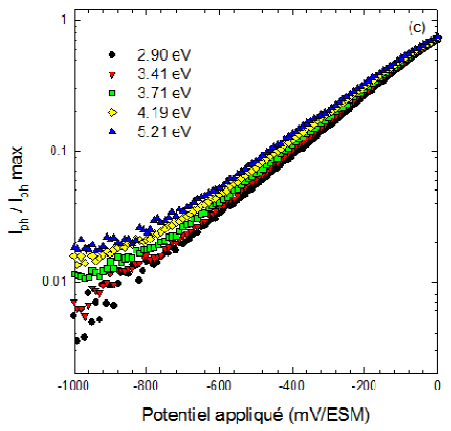
\includegraphics[width=0.65\textwidth]{./src/figures/Loucif2012-Fig3-19.png}
                \caption{}
                \label{fig_loucif_sctype_b}
            \end{subfigure}
            
            %\caption{Photocurrent with respect to the potential for an 
            %Ni-based alloy 600 polished and oxidized in simulated PWR 
            %for 500~h \citep{loucif2013}: a) $P_{H_2}$=6.5~bar, b) $P_{H_2}$=0.05~bar.}
            \label{fig_loucif_sctype}
        \end{figure}
    \end{frame}

\subsection{High temperature PEC}
    \begin{frame}[allowframebreaks=1.0]{High temperature PEC}
        \begin{itemize}
            \item The majority of photoelectrochemical characterizations are performed at 
            room temperature in simple glass/Plexiglas cells where the signal/noise 
            ratio is very good.
            \item High temperature photoelectrochemical characterizations 
            require sophisticated metallic cells and transparent windows 
            able to withstand the arch environment. 
            \item Despite the need to improve the signal/noise ratio, the feasibility of 
            the in-situ photoelectrochemical characterizations was demonstrated by 
            \citet{bojinov2002} in 2002 and more recently by \citet{skocic2016} in 2015 
        \end{itemize}

        \renewcommand{\coef}{0.45}
        \begin{figure}[h]
            \centering
            \begin{subfigure}{\coef\textwidth}
                \centering
                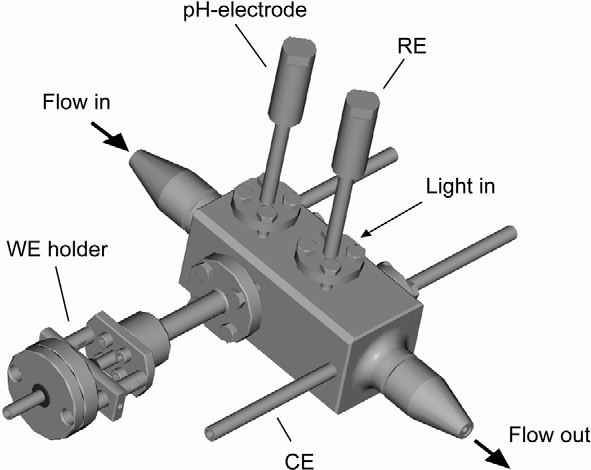
\includegraphics[width=\textwidth]{./src/figures/Bojinov_2002_Fig1.png}
                \caption{}
                \label{fig_bojinov_ht_a}
            \end{subfigure}
            \begin{subfigure}{\coef\textwidth}
                \centering
                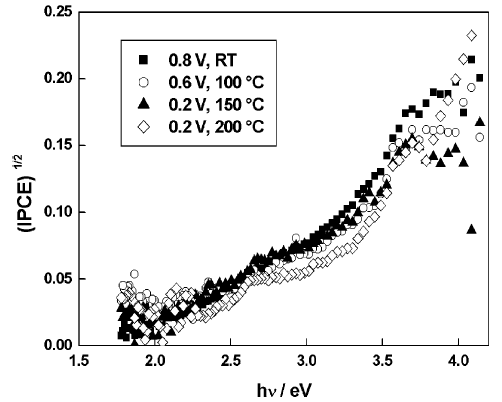
\includegraphics[width=\textwidth]{./src/figures/Bojinov_2002_Fig5b.png}
                \caption{}
                \label{fig_bojinov_ht_b}
            \end{subfigure}
            
            %\caption{a) Schematic representation of the metallic cell developed
            %by \citet{bojinov2002}. 
            %b) Photocurrent spectra performed on iron oxides at different 
            %temperatures (up to 200°C) obtained by \citet{bojinov2002}.}
            \label{fig_bojinov_ht}
        \end{figure}

        \renewcommand{\coef}{0.45}
        \begin{figure}[h]
            \centering
            \begin{subfigure}{\coef\textwidth}
                \centering
                \includegraphics[width=\textwidth]{./src/figures/skocic2015-1.png}
                \caption{}
                \label{fig_skocic_phd_cell}
            \end{subfigure}
            \begin{subfigure}{\coef\textwidth}
                \centering
                \includegraphics[width=\textwidth]{./src/figures/skocic2015-2.png}
                \caption{}
                \label{fig_skocic_phd_htpec}
            \end{subfigure}
            
            %\caption{a) Schematic view of the photoelectrochemical cell developed by \citet{skocic2016}. 
            %b) Photocurrent energy spectra of an X750 specimen recorded at room
            %temperature and in 280°C/80 bar water \citep{skocic2016}}
            \label{fig_skocic_phd}
        \end{figure}
    \end{frame}




% BIBLIOGRAPHY
\begin{frame}[allowframebreaks=0.9]{References}
\AtNextBibliography{\tiny}
\nocite{*}
\printbibliography
\end{frame}

\end{document}
